\documentclass{standalone}

\usepackage{tikz}
\usepackage{libertine}

\begin{document}

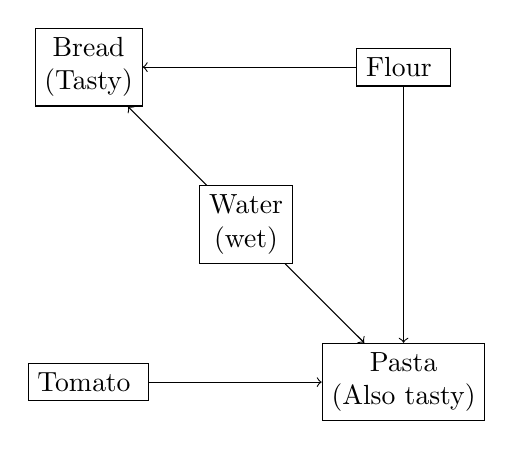
\begin{tikzpicture}[scale=2]
  \tikzstyle{mynode}=[draw, rectangle,align=center]

  \node[mynode] (Bread) at (-1, 1) { Bread\\(Tasty)};

  \node[mynode] (Flour) at (1, 1) { Flour };

  \node[mynode] (Water) at (0, 0) { Water\\(wet)};

  \node[mynode] (Tomato) at (-1, -1) { Tomato };

  \node[mynode] (Pasta) at (1, -1) { Pasta\\(Also tasty) };

  \draw[->] (Flour) -- (Bread);
  \draw[->] (Water) -- (Bread);

  \draw[->] (Flour) -- (Pasta);
  \draw[->] (Water) -- (Pasta);

  \draw[->] (Tomato) -- (Pasta);

\end{tikzpicture}

\end{document}
